\subsubsection{First Level Track Jet Trigger for Displaced Jets at High Luminosity LHC}

The high luminosity LHC program offers many exciting opportunities to search for rare processes. It is expected that the
LHC will accumulate 3\abinv of proton-proton collisions at 14\UTeV.
The CMS detector will undergo major upgrades to all subsystems, including the tracker~\cite{cmstdr-014},
the barrel~\cite{cmstdr-barrel} and endcap~\cite{cmstdr-ec} calorimeters, the muon system~\cite{cmstdr-mu},
and the trigger~\cite{cmstdr-017}. 

The bandwidth limitations of the first level (L1) trigger
are one of the main problems facing current searches 
for exotic Higgs boson decays, as well as many other signals beyond the standard model.
The process where the Higgs boson decays to two new light scalars that in turn decay to jets, \Hphiphi, is an important example. If the scalar $\phi$ has a
macroscopic decay length, the offline analysis has no background from SM processes, but the majority of the signal events do not get recorded because they fail to be selected by the L1 trigger.
The main obstacle is the high rate for low transverse momentum jets, which is made worse by additional extraneous \pp collisions in the
high luminosity environment.

In this note~cite{CMS-PAS-FTR-18-018}, we investigate the capabilities of L1 track finding~\cite{cmstdr-014} to increase the L1 trigger efficiency for such signals.
We focus on small or moderate decay lengths of the new particles, 1--50\Umm, and assume, as is demonstrated by
many analyses~\cite{ll1, ll2, ll3}, that the offline selection can remove all SM backgrounds with only a moderate loss of efficiency.

The investigation has two major thrusts. First, we propose a jet clustering algorithm that uses the L1 tracks found with a primary vertex constraint.
Second, we consider the extension of the L1
track finder to off-pointing tracks, and develop a jet lifetime tag for tracks with $|\eta| < 1.0$. 
Future work will include: expanding the off-pointing track finding at L1 to the full acceptance of the outer tracker;
matching the track jets with high transverse energy (\ET) deposits in the electromagnetic calorimeter; and finding new ways to evaluate
track quality to suppress ``fake'' tracks that result from finding the wrong combination of track hits. 

While in this study we focus on the specific Higgs boson decay to light scalars (see Ref.~\cite{bsmh} for extensive review of physics motivations for such decays),
the results and the proposed triggers are relevant for a broad spectrum of new physics searches, with or without macroscopic decay lengths.

\paragraph{Signal and background simulation}

In these studies, the Phase-2 CMS detector is simulated using \GEANTfour~\cite{geant}.
Event samples corresponding to 200 collisions per bunch crossing (pileup) \cite{cmstdr-017} are used for the evaluation of trigger rates.

The following signal samples are considered:
\begin{enumerate}
\item Displaced single muons, generated with a uniform distribution of transverse momentum (\pt) between 2 and 8\UGeV, uniform
in $\eta$ between -1 and 1, and with impact parameter \dtrans distributed as a Gaussian with width $\sigma=2\Ucm$.
\item The decay of the SM Higgs boson $\PH(125)\to \phi\phi\to \bbbar\bbbar$, with $\phi$ masses of 15, 30, and 60\UGeV, and \ctau of 0, 1, and 5\Ucm.
The production of the Higgs boson via gluon fusion is simulated by \POWHEG v2.0 \cite{powheg}, while the hadronization and decay is performed by \PYTHIA v8.205 \cite{pythia}.
\item The decay of a heavy SM-like Higgs boson with mass 250\UGeV, $\PH(250)\to \phi\phi\to \bbbar\bbbar$, with $\phi$ masses of 15, 30, and 60\UGeV, and \ctau of 0, 1, and 5\Ucm.
The production of the heavy SM-like Higgs boson via gluon fusion, its decay, and its hadronization are all simulated with \PYTHIA 8 \cite{pythia}.
\end{enumerate}

\paragraph{Track jets}
\label{sec:trackjets}

The tracker is the most granular detector participating in the L1 decision, and therefore the most resilient to pileup. 
Track finding at L1 relies on selection at the front end of tracker hits that originated from high transverse momentum particles.
This is achieved through use of the so-called \pt-modules consisting of two sensors separated by a few mm \cite{cmstdr-014}. A particle crossing a tracker module
produces a pair of hits in the two sensors. Such pairs form a ``stub'' if the azimuthal difference between the hits in the two sensors of a module is consistent
with a prompt track with $\pt \gtrsim 2\UGeV$.

In this section, we describe a simple jet clustering algorithm implementable in firmware, and compare it with anti-\kt jets~\cite{Cacciari:2008gp} with a size parameter of $R = 0.3$,
as produced by \FASTJET~\cite{fastjet}.

A simplified algorithm for L1 track jets is used to facilitate the firmware implementation for the L1 trigger applications. 
L1 track jets are found by grouping tracks in bins of \zo, the point of closest approach to the $z$-axis, for the tracks. The bins are overlapping, staggered by
half a bin, so that each track ends up in two bins, eliminating inefficiencies at bin edges. In each \zo bin, the \pt of the tracks are summed in bins of
$\eta$ and azimuthal angle $\phi$ with bin size $0.2 \times 0.23$. A simplified nearest-neighbor clustering is performed, and the total $\HT=\sum \pt^{\text{trk}}$ in the \zo bin is calculated.
The \zo bin with the highest \HT is chosen. Jets obtained through this algorithm are referred to as ``TwoLayer Jets.'' 
For the studies below, \zo bins with size 6 cm are used. Jets with $\ET>50\,(100)\UGeV$ are required to have at least two (three) tracks.


The track purity depends on the number of stubs in the track and the $\chi^2$ of the track fit. High-\pt tracks are much less pure than low-\pt tracks,
with fake tracks distributed approximately uniformly in $1/\pt$ while real tracks are mostly low-\pt.
To mitigate the effect of high-\pt fake tracks, any track with a reconstructed \pt above 200\UGeV is assigned a \pt of 200\UGeV. The track quality selection used in this analysis
is summarized in Table~\ref{tab:tracksel}. 

\begin{table*}[htb]
\centering
\caption{Track selection for jet finding. The $\chi^2$ selections are per degree of freedom for a 4-parameter track fit. \label{tab:tracksel}}
\begin{tabular}{r|ccc}
\hline
track \pt & 4 stubs  & 5 stubs & 6 stubs \\
\hline
2--10\UGeV   & $\chi^2<15$ & $\chi^2<15$ & accept \\
10--50\UGeV & reject      & $\chi^2<10$ & accept \\
${>}50\UGeV$   & reject      & $\chi^2<5$ & $\chi^2<5$ \\
\hline
\end{tabular}
\end{table*}


We have verified that the TwoLayer trigger algorithm gives similar performance to a full jet clustering using the anti-\kt algorithm with a size parameter $R = 0.3$, as implemented in \FASTJET.
Figure~\ref{fig:jeteff} shows the efficiency to reconstruct a track jet as function of the generator-level jet \pt.
Figure~\ref{fig:rates} shows the calculated L1 trigger rates for an \HT trigger (scalar sum of \pt of all jets above threshold)
and a quad-jet trigger (at least four jets above threshold) as a function of the threshold.
\HT is computed from track jets with $\pt>5\UGeV$.

The rates are computed based on a fixed number of colliding bunches. The trigger rate is computed as
\begin{equation*}
  \text{Rate} = \effLT \Nbunches \fLHC,
\end{equation*}
where $\Nbunches=2750$ bunches for 25\Uns bunch spacing operation, $\fLHC = 11246\UHz$, and \effLT is the efficiency to pass a given L1 threshold as determined
in simulation. For both the L1 trigger efficiency and rate, the performance of the TwoLayer hardware algorithm is compatible with the performance from the more sophisticated algorithm
from \FASTJET.

\begin{figure*}[hbtp]\centering
 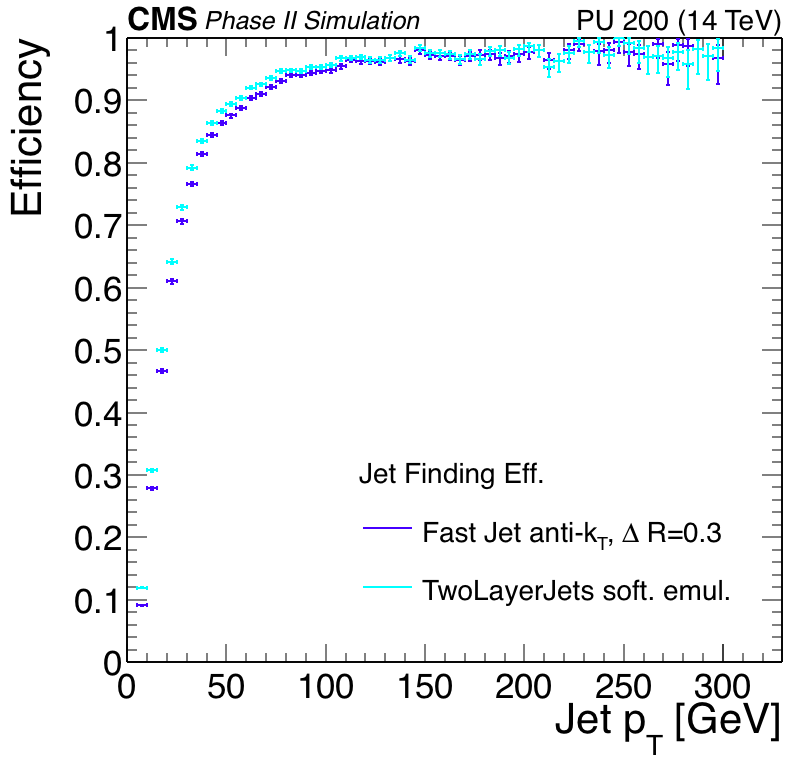
\includegraphics[width=0.45\textwidth]{\main/section9/plots/jet_eff.png}
 \caption{The efficiency for a jet to give rise to a L1 track jet as a function of the generator-level \pt of the jet.
 The light and dark blue lines correspond to the trigger clustering (TwoLayer Jets) and anti-\kt with $R =0.3$ (\FASTJET), respectively.}
  \label{fig:jeteff}
\end{figure*}%

\begin{figure*}[hbtp]\centering
 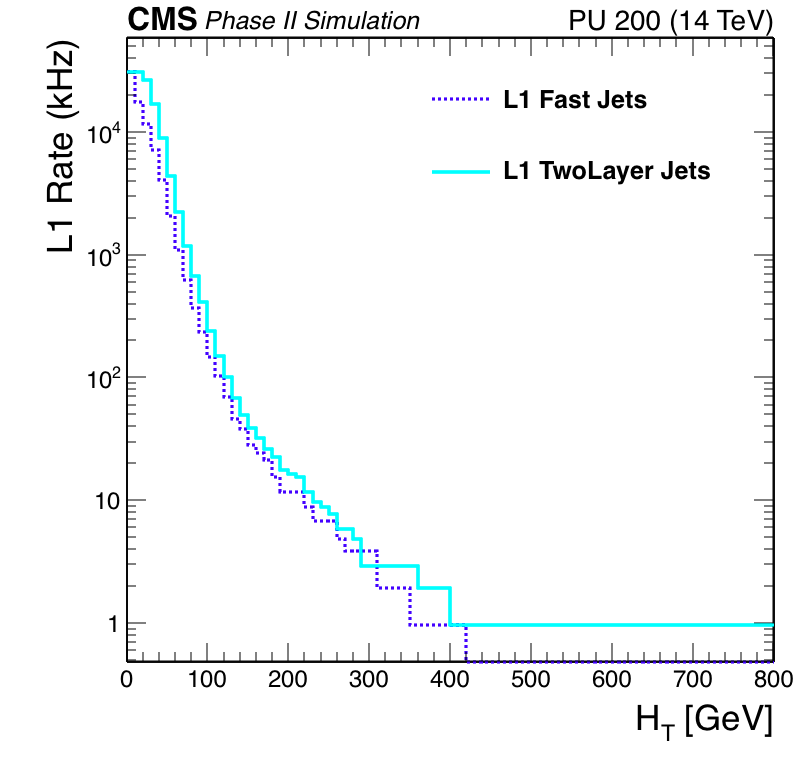
\includegraphics[width=0.45\textwidth]{\main/section9/plots/rates_HT.png}
 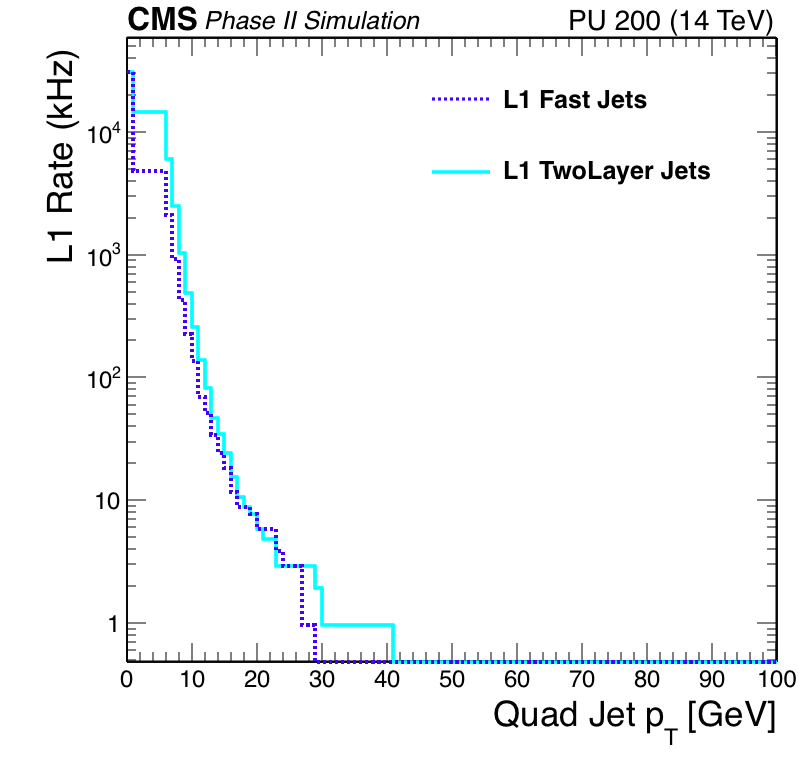
\includegraphics[width=0.45\textwidth]{\main/section9/plots/rates_Quad.png}
 \caption{Calculated L1 trigger rates for track jet based \HT (left) and quad-jet (right) triggers.
 The light and dark blue lines correspond to the trigger clustering (TwoLayer Jets) and anti-\kt with $R =0.3$ (\FASTJET), respectively.}
  \label{fig:rates}
\end{figure*}%

\paragraph{Displaced track finding}

In this section, we briefly describe the performance of an algorithm for reconstruction of tracks with non-zero impact parameter. This approach extends the baseline L1 Track Trigger design to 
handle tracks with non-zero impact parameter and to include the impact parameter in the track fit. This enhanced design is feasible without greatly altering the track finding approach, but will 
require more computational power than the current proposal, which considers only prompt tracks. Tracks passing the selection are clustered using the same algorithm as described in Section~\ref{sec:trackjets}, 
and clusters containing tracks with high impact parameters are flagged as displaced jets. Though the baseline design of the L1 Track Trigger currently is optimized to find prompt tracks, these 
studies show that an enhanced L1 Track Trigger can extend the L1 trigger acceptance to include new BSM physics signals.

\begin{figure*}[hbtp]\centering
 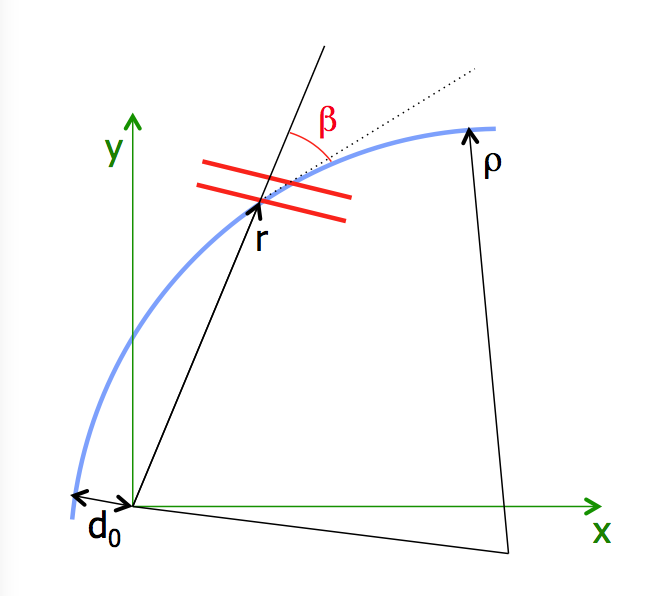
\includegraphics[width=0.49\textwidth]{\main/section9/plots/bends.png}
 \caption{A sketch of a track crossing a \pt-module.}
  \label{fig:bend}
\end{figure*}%

A track with a sufficiently small impact parameter can produce a stub.
For tracks with large \pt (i.e. large curvature radius $\rho$) and small \dtrans,
the bending angle $\beta$ between the track and the prompt infinite momentum track, as shown in Fig. \ref{fig:bend}, is
\begin{equation*}
  \beta \approx \frac{r}{2\rho} - \frac{\dtrans}{r}.
\end{equation*}

Therefore, for a given \dtrans, one expects the stubs to be formed more efficiently as the radius of the module $r$ increases.
Fig. \ref{fig:stubeff} shows the efficiency for a displaced muon to produce a stub as a function of the signed transverse momentum and the impact parameter
of the muon, as measured in the full \GEANTfour-based simulation of the Phase-2 detector. 

\begin{figure*}[hbtp]\centering
 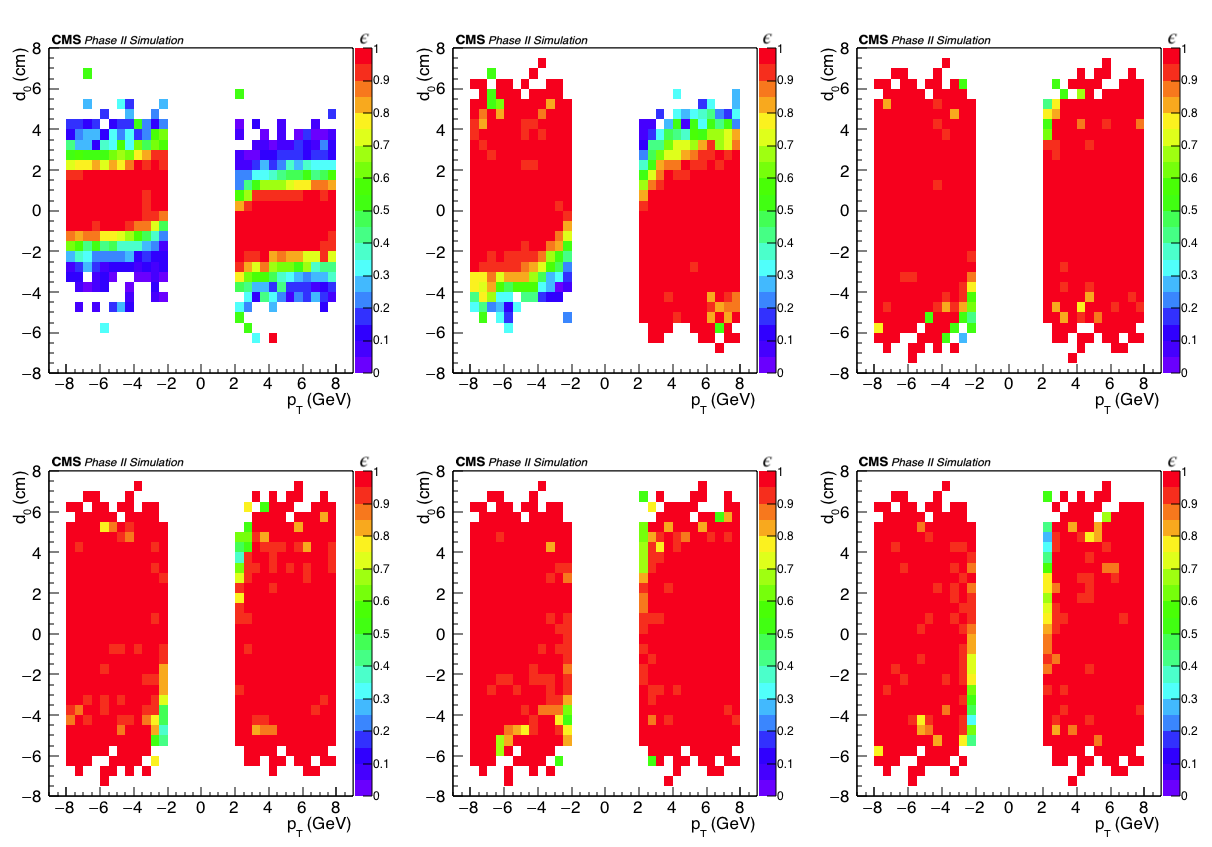
\includegraphics[width=0.9\textwidth]{\main/section9/plots/stubeff_d0.png}
 \caption{The efficiency for a displaced muon to form stubs in the six barrel layers of the Phase-2 tracker, as a function of the signed muon \pt and impact parameter.
 The top row shows, from left to right, layers 1, 2, and 3;
 the bottom row shows layers 4, 5, and 6.
 The sample is comprised of 2000 muons generated with uniformly distributed transverse momentum between 2 and 8\UGeV and pseudorapidity $|\eta|<1$, and with the impact parameter \dtrans
 distributed as a Gaussian with width of 2\Ucm.}
  \label{fig:stubeff}
\end{figure*}

A special version of the tracklet algorithm \cite{cmstdr-014} has been developed that is capable of reconstructing tracks with impact parameters of a few cm.
For now, the reconstruction is limited to the barrel region ($|\eta|<1.0$). Preliminary feasibility studies show
that the algorithm will have similar performance in the entire outer tracker coverage. 

Fig. \ref{fig:trackeff} shows the track reconstruction efficiency requiring at least four and at least five stubs on the track. As expected, allowing
only four stubs on a track gives a higher efficiency for high impact parameter tracks.

\begin{figure*}[hbtp]\centering
 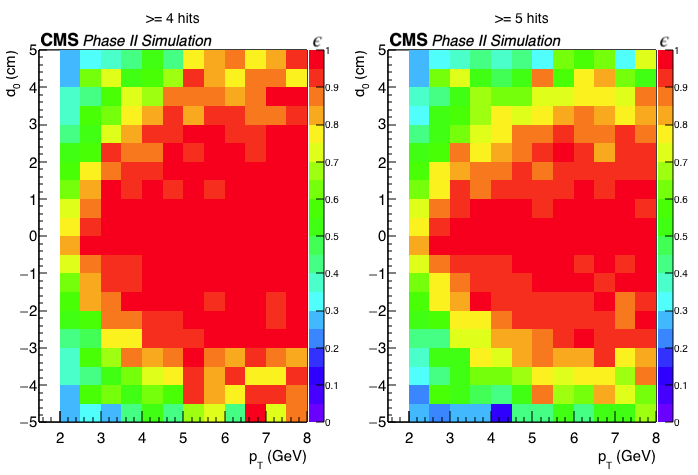
\includegraphics[width=0.9\textwidth]{\main/section9/plots/trackeff_d0.png}
 \caption{The efficiency for a displaced muon to be reconstructed as a track with at least four stubs (left) and at least five stubs (right).}
  \label{fig:trackeff}
\end{figure*}%

For the extended track finding algorithm, two track fits are performed:
a 3-parameter $r\phi$ fit yielding $1/\rho$, $\phi_0$, and \dtrans, and a 2-parameter $rz$ fit
yielding $t$ and \zo. The bend consistency variable is defined as
\begin{equation*}
\text{consistency} = \frac{1}{\Nstubs} \sum_{i=1}^{\Nstubs}\left(\frac{\beta_i - \beta_i^{\text{exp}}}{\sigma_{i}}\right)^2,
\end{equation*}
where \Nstubs is the total number of stubs comprising the track, $\beta_i$ and $\beta_i^{\text{exp}}$ are the measured and expected bend angles for stub $i$,
and $\sigma_i$ is the expected bend angle resolution.

Two track categories are defined, loose and tight.
The selection is summarized in Table \ref{tab:dtracksel}.

\begin{table*}[htb]
\centering
\caption{Track selection criteria for jet finding with extended L1 track finding. \label{tab:dtracksel}}
\begin{tabular}{c|ccc|ccc}
\hline
           & \multicolumn{3}{c|}{Loose}                        & \multicolumn{3}{c}{Tight} \\
           %\cline{2-7}
\Nstubs & $\chi^2_{r\phi}$ & $\chi^2_{rz}$ & consistency & $\chi^2_{r\phi}$ & $\chi^2_{rz}$ & consistency \\
\hline
$4$      &  ${<}0.5$ & ${<}0.5$ & ${<}1.25$ & \multicolumn{3}{c}{reject} \\
$\geq 5$ &  ${<}5.0$ & ${<}2.5$ & ${<}5.0$  & ${<}3.5$ & ${<}2.0$ & ${<}4.0$ \\
\hline
\end{tabular}
\end{table*}

A jet is required to have at least two tracks passing the tight selection. If two or more tight tracks
in a jet have $|\dtrans|>0.1\Ucm$, the jet is tagged as a displaced jet.

\paragraph{Results}

Figure \ref{fig:reff} shows the rate of the track jet \HT trigger as a function of the efficiency
of the heavy SM-like Higgs boson signal. While for prompt $\phi$ decays one can realistically achieve 20\%
efficiency at an L1 rate of 25\UkHz, the efficiency quickly drops with the decay length, since the displaced tracks are not reconstructed for \dtrans values above a few mm.

\begin{figure*}[hbtp]\centering

 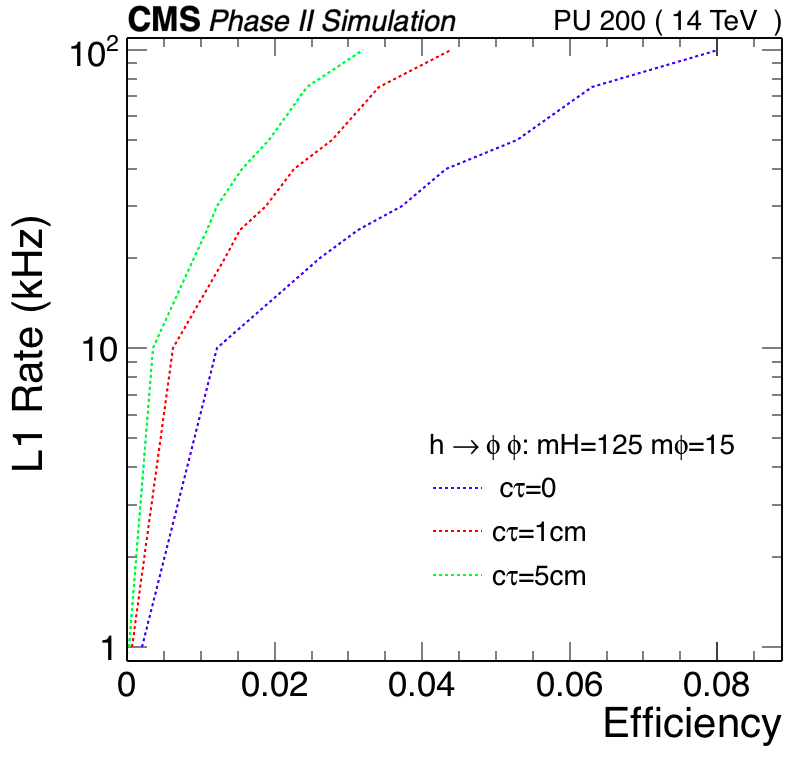
\includegraphics[width=0.49\textwidth]{\main/section9/plots/reff_h125.png}
 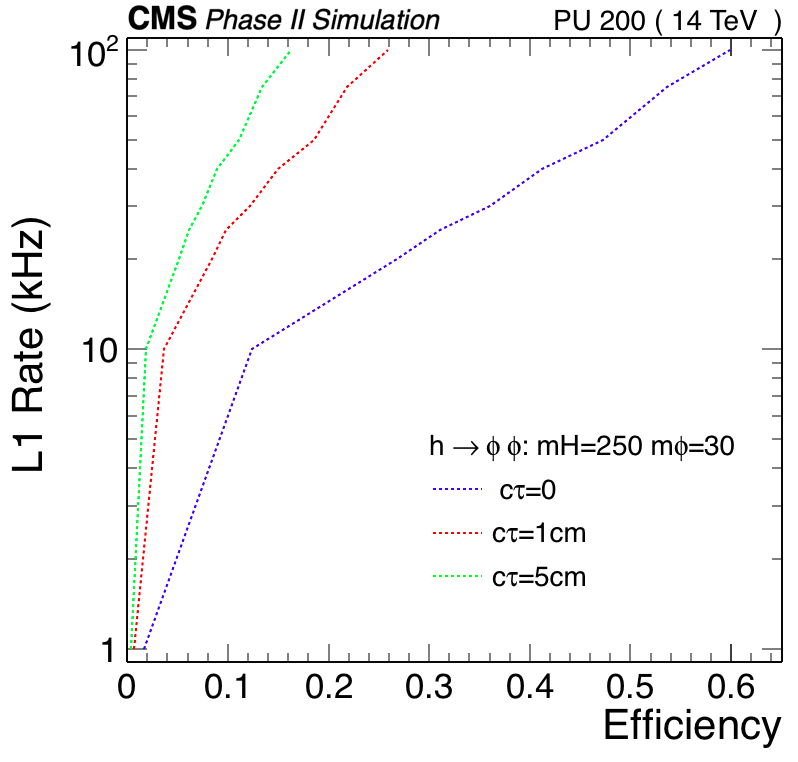
\includegraphics[width=0.49\textwidth]{\main/section9/plots/reff_h250_mphi30.png} \\
 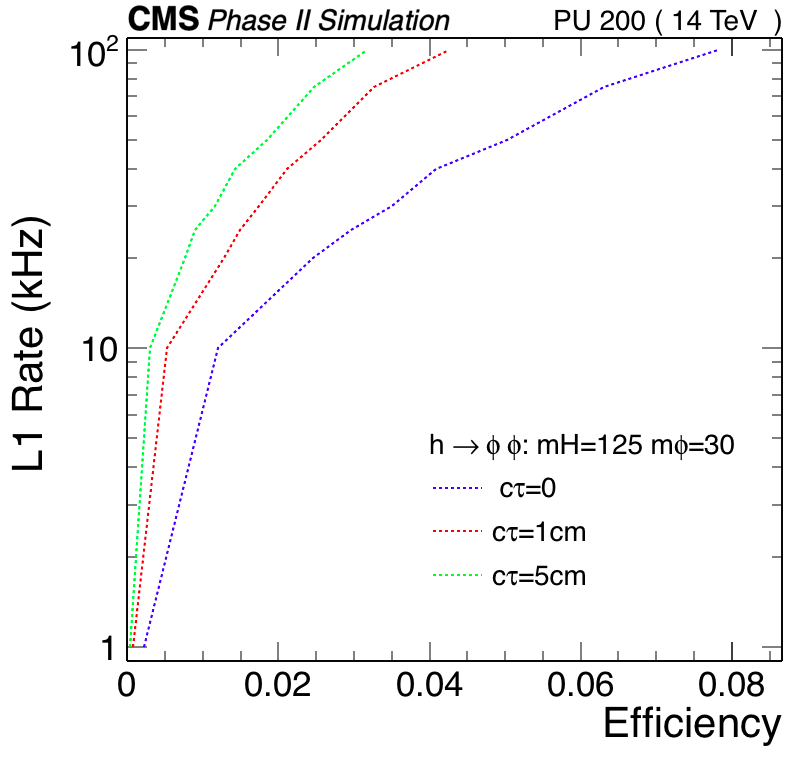
\includegraphics[width=0.49\textwidth]{\main/section9/plots/reff_h125_mphi30.png}
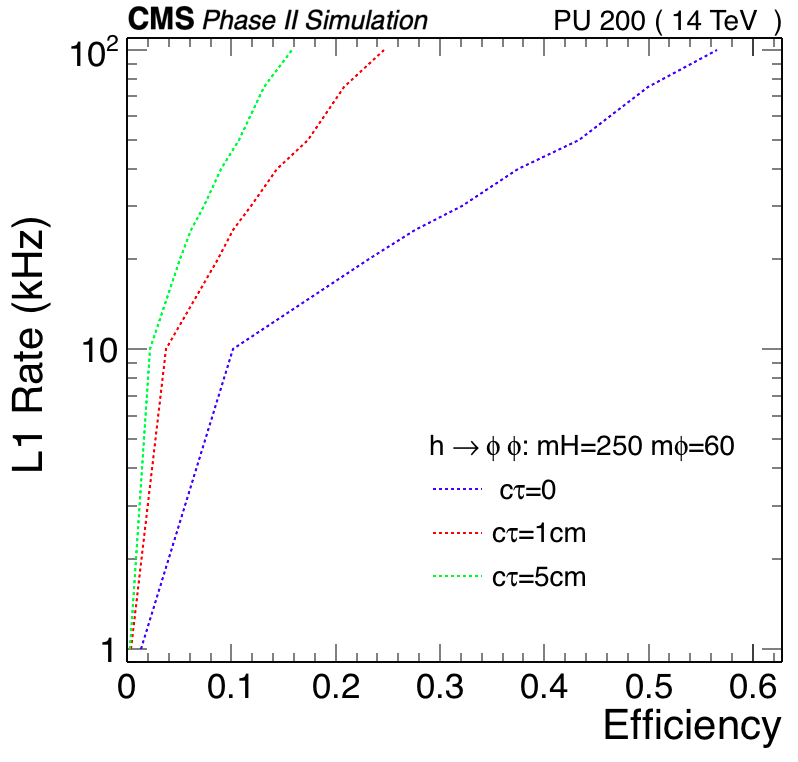
\includegraphics[width=0.49\textwidth]{\main/section9/plots/reff_h250.png}
 \caption{The rate of the track jet \HT trigger as a function of signal efficiency for the SM Higgs boson (left) and the heavy SM-like Higgs boson (right) using prompt track finding.}
  \label{fig:reff}
\end{figure*}%

The rate for the \HT trigger using the extended track finding is shown in Fig. \ref{fig:rate_disp}, with and without 
a requirement of at least one jet with a displaced tag. The displaced tag requirement suppresses the rate by more than
an order of magnitude. The displaced tracking and the trigger that requires a jet with a displaced tag make the signals with low \HT accessible for displaced jets.

\begin{figure*}[hbtp]\centering
 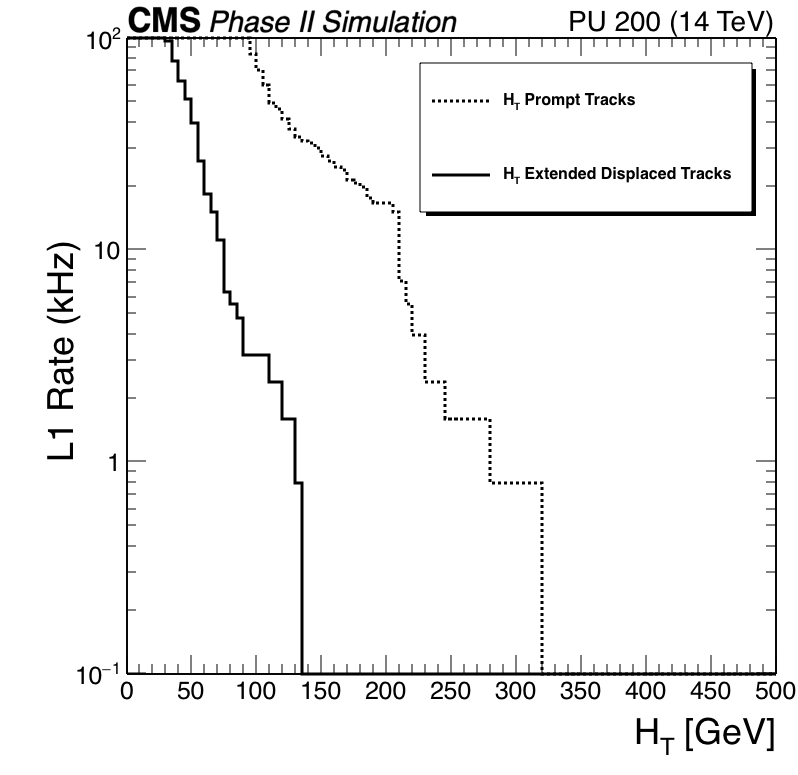
\includegraphics[width=0.49\textwidth]{\main/section9/plots/rate_disp.png}
 \caption{The rate of the track jet \HT trigger using extended track finding with (solid line) and without (dashed line) a
 requirement of at least one jet with a displaced tag.}
  \label{fig:rate_disp}
\end{figure*}

In order to compare the results with prompt and extended track reconstruction, one needs to make a correction for
the rapidity coverage: prompt tracks are found in $|\eta|<2.4$, while the extended track algorithm currently only
reconstructs tracks in $|\eta|<1.0$.  For the feasible thresholds, the rate for $|\eta|<0.8$ and $|\eta|<2.4$ differ by a factor of five.  To scale the efficiency for finding track jets to the full
$|\eta|<2.4$ range, we derive a scale factor (SF) based on efficiency in the full $\eta$ range and the central $\eta$ range. The signal efficiency SFs range from 4--6, 
which is comparable to the increase in the L1 rate.
We have confirmed that such extrapolation works for the track jets clustered with prompt tracks. Figure \ref{fig:reff_dispextra} shows the expected trigger rate as a function of efficiency for the SM and the heavy SM-like Higgs bosons.

\begin{figure}[hbtp]
  \centering
    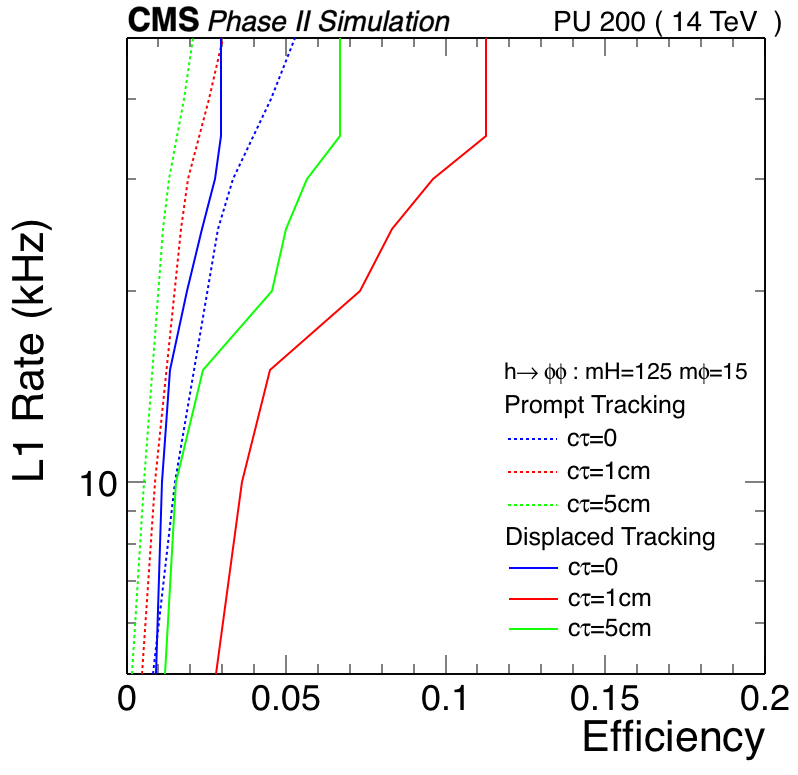
\includegraphics[width=0.49\textwidth]{\main/section9/plots/ExtrapolatedRatemH125_mPhi15.png}
    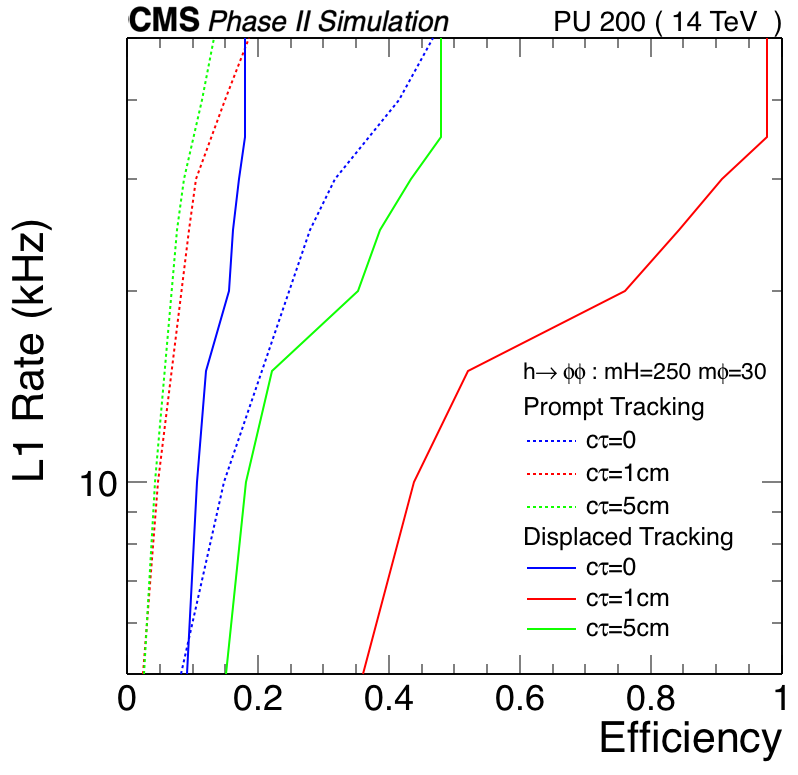
\includegraphics[width=0.49\textwidth]{\main/section9/plots/ExtrapolatedRatemH250_mPhi30.png}\\
    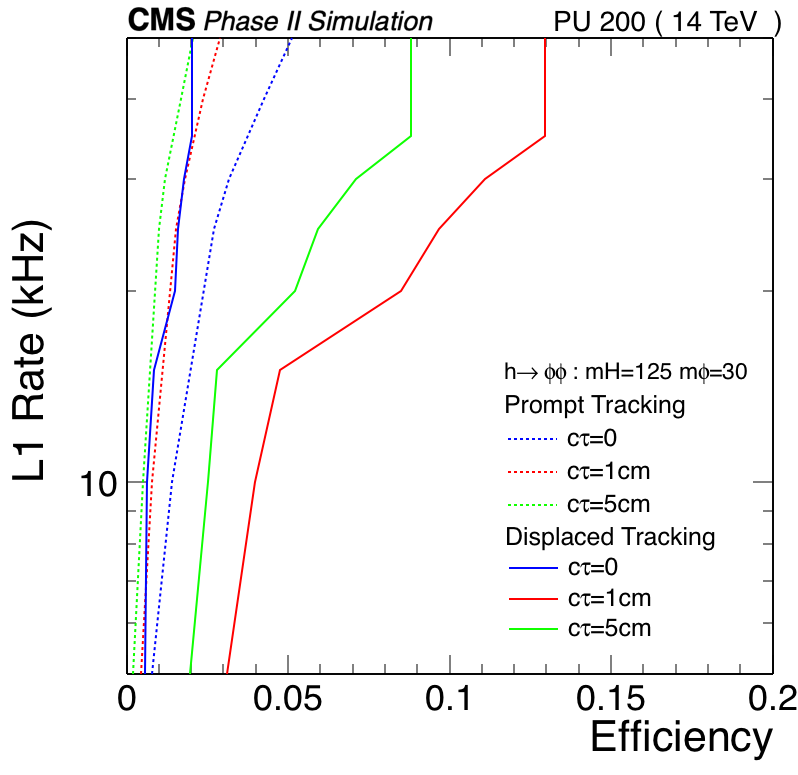
\includegraphics[width=0.49\textwidth]{\main/section9/plots/ExtrapolatedRatemH125_mPhi30.png}
    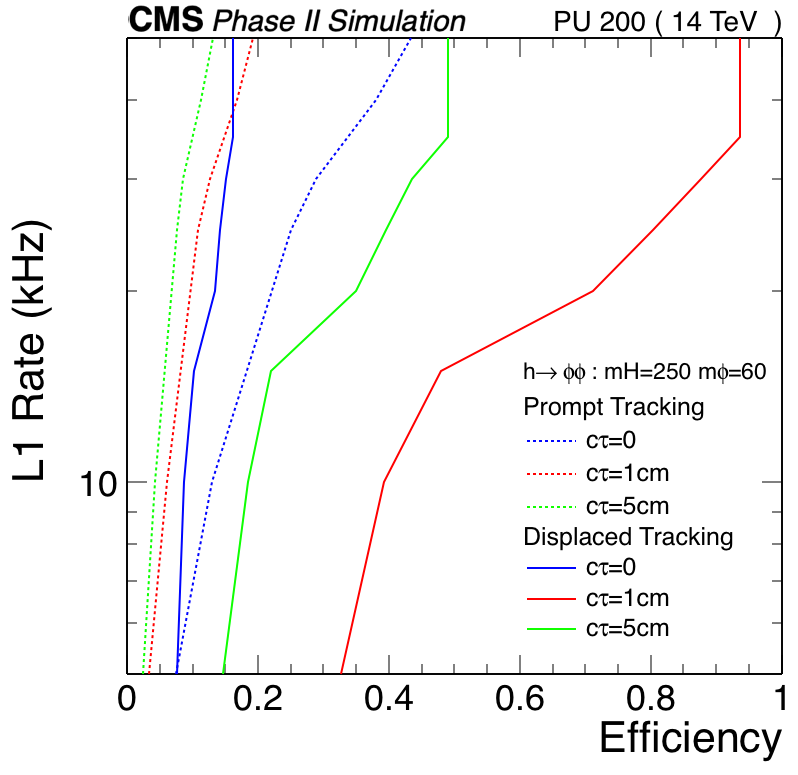
\includegraphics[width=0.49\textwidth]{\main/section9/plots/ExtrapolatedRatemH250_mPhi60.png}
    \caption{The rate of the track jet \HT trigger as a function of signal efficiency using extended track finding for the SM Higgs (left)
    and the heavy SM-like Higgs (right). The extended track finding performance is extrapolated to the full outer tracker acceptance as described in text.}
    \label{fig:reff_dispextra}
\end{figure}

The available bandwith for the triggers described above, if implemented, will be decided as a part of the full trigger menu optimization.
Here, we consider two cases, 5 and 25\UkHz. The expected event yield for triggers using extended and prompt tracking are shown in Fig. \ref{fig:money},
assuming branching fraction $\mathcal{B}[\Hphiphi] = 10^{-5}$ for the SM Higgs boson.
For the heavy Higgs boson, the expected number of produced signal events is set to be the same as for the SM Higgs by requiring
$\sigma_{\pp\to \PH(250)} \mathcal{B}[\BSMHphiphi] = 10^{-5} \sigma_{\pp\to \PH(125)}$.

\begin{figure}[hbtp]
  \centering
    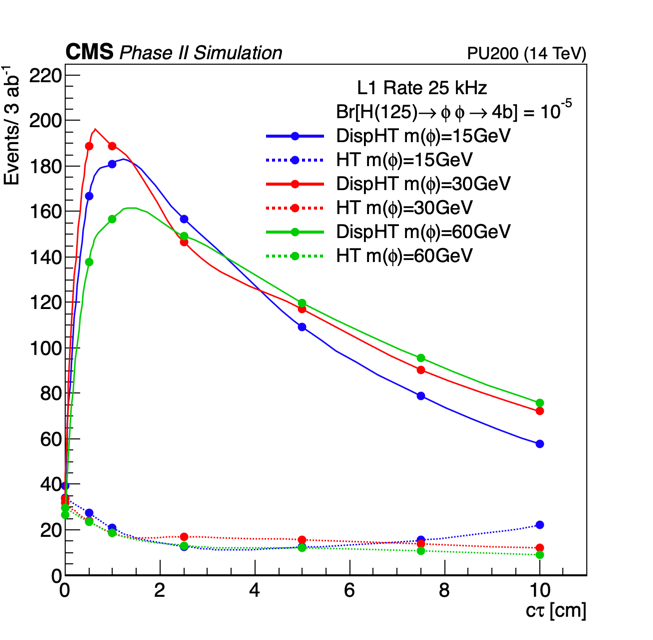
\includegraphics[width=0.49\textwidth]{\main/section9/plots/HiggsM125_25kHzYieldsvsLifetime.png}
    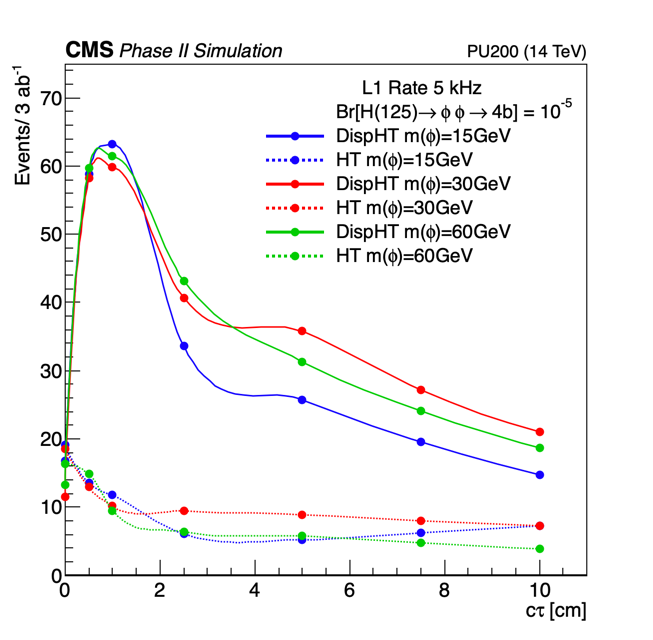
\includegraphics[width=0.49\textwidth]{\main/section9/plots/HiggsM125_5kHzYieldsvsLifetime.png}\\
    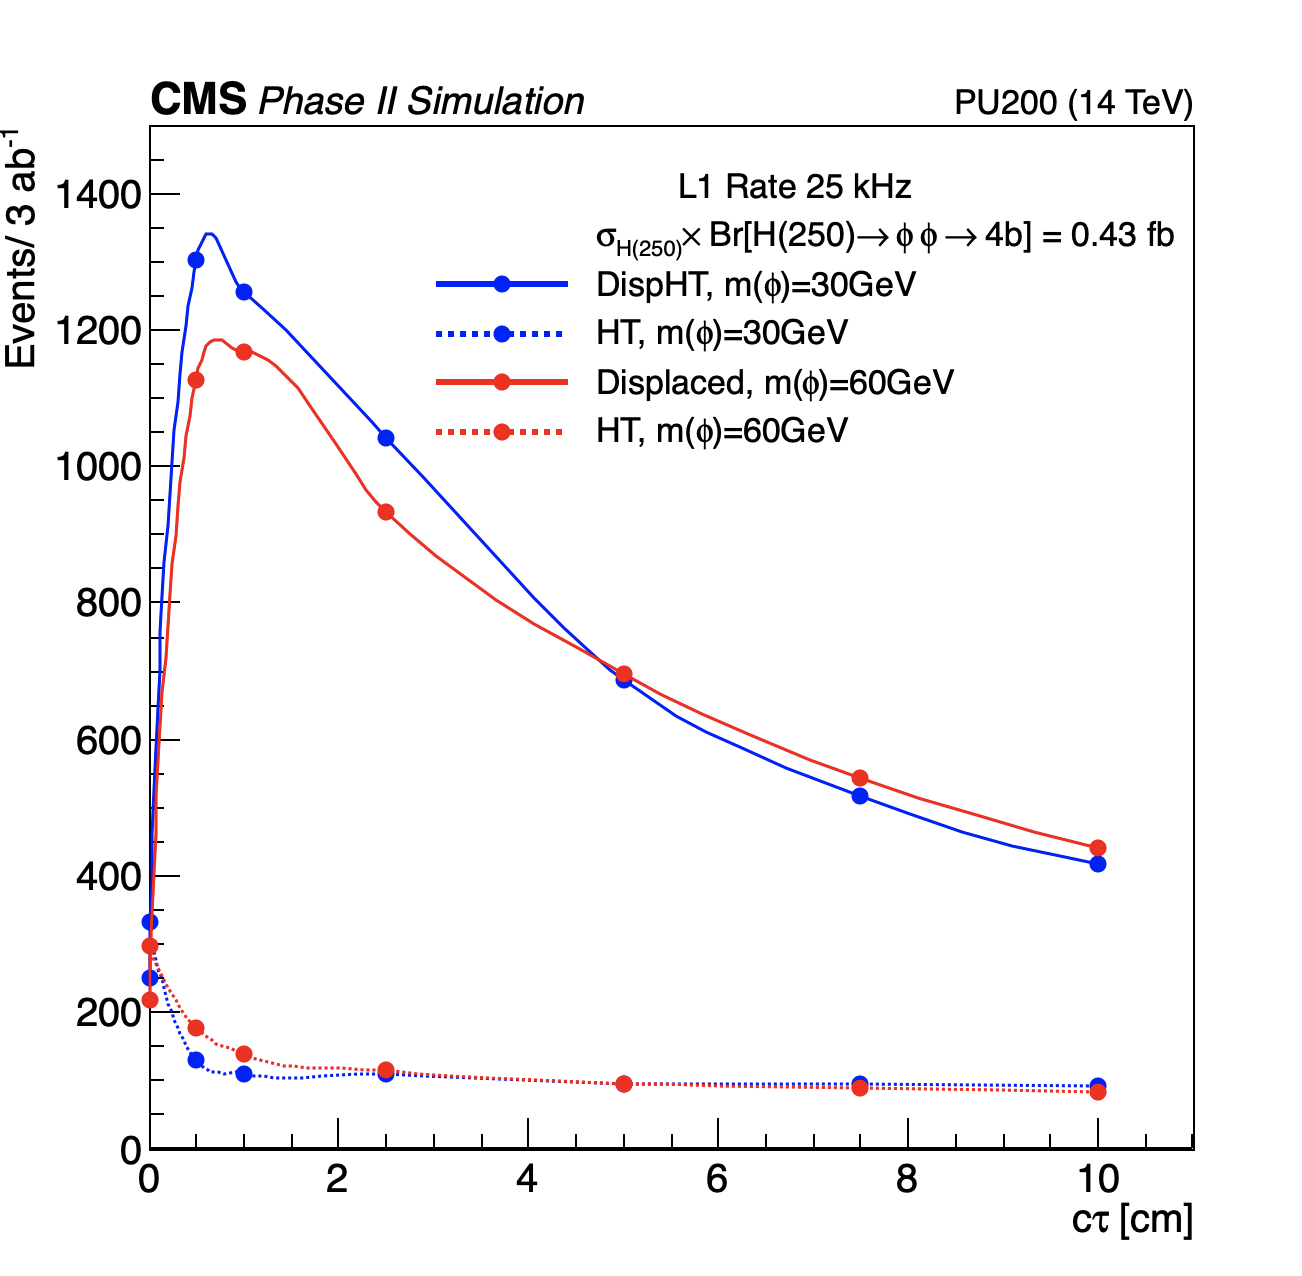
\includegraphics[width=0.49\textwidth]{\main/section9/plots/HiggsM250_25kHzYieldsvsLifetime.png}
    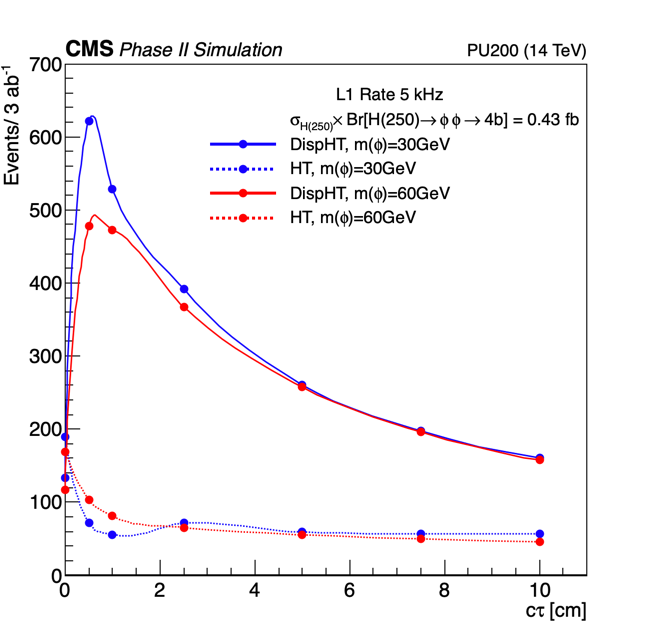
\includegraphics[width=0.49\textwidth]{\main/section9/plots/HiggsM250_5kHzYieldsvsLifetime.png}
    \caption{This plot shows the number of triggered Higgs events (assuming ${\mathcal{B}[\Hphiphi] = 10^{-5}}$, corresponding to 
1700 events) as a function of \ctau for two choices for the trigger rates: 25\UkHz (left), 5\UkHz (right).
Two triggers are compared: one based on prompt track finding (dotted lines) and another that is based on extended track finding 
with a displaced jet tag (solid lines). }
    \label{fig:money}
\end{figure}

\paragraph{Conclusion}

We have studied the upgraded CMS detector's ability to trigger on events with long lived particles decaying into jets.
Currently, such events pass the L1 trigger only if the total transverse energy in the event is above a few hundred \UGeV.
This is an important blind spot for searches, especially for the rare exotic Higgs boson decays like
 \Hphiphi.

In this note, a new L1 trigger strategy based on the Phase-2 CMS detector's ability to find tracks at L1 is explored.
Using L1 tracks for jet reconstruction significantly suppresses pile-up and allows to accept events with lower \HT.
For the exotic Higgs decays considered, given the total Phase-2 dataset of 3\abinv and branching fraction of $10^{-5}$, 
CMS would collect $\mathcal{O}(10)$ events, which should be sufficient for discovery.
We also considered a plausible extension of the L1 track finder to consider tracks with impact parameters of a few cm.
That approach improves the yield by more than an order of magnitude. The gains for the extended L1 track finding
are even larger for the events with larger \HT, as demonstrated by the simulations of heavy Higgs boson decays.

